\newpage
\section{Implementierung PWA}
Schritte der Implementierung
\begin{enumerate}
	\item Einrichten der Entwicklungsumgebung
	\item Initialisierung des Projekts
	\item Installation der Pakete
\end{enumerate}

\subsection{Einrichten der Projektumgebung}
Für die Entwicklung der PWA wird die Entwicklungsumgebung Webstorm von JetBrains gewählt, da sie die viele Routineaufgaben selbstständig beziehungsweise mit geringem Aufwand ausführt. 

Wie für die Entwicklung der meisten modernen Webanwendungen ist die Installation der Node.js Laufzeitumgebung notwendig. Mit dem integrierten Paketmanager npm lassen sich Bibliotheken leicht zum Projekt hinzufügen.
Um die Angular Anwendung automatisiert zu erstellen, ist zuerst die Installation des Angular \acf{cli} erforderlich. Mit dem Konsolenbefehl \texttt{npm install -g @angular/cli} wird npm aufgefordert, die neuste Version der Angular CLI global auf dem System zu installieren.


Mit dem Befehl \texttt{ng new todoapp} wird die Angular CLI (in der Konsole als \texttt{ng} abgekürzt) dazu gebracht, ein Angularprojekt inklusive nötiger Dateistrukturen zu erstellen. 
\begin{wrapfigure}{r}{0.6\textwidth}
	\vspace{-10pt}
	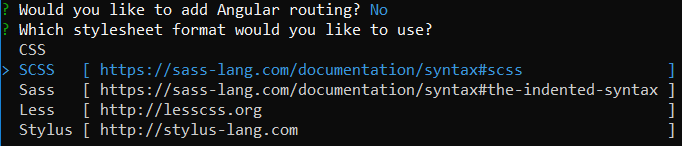
\includegraphics[width=0.58\textwidth]{img/angular_cli_css.PNG}
	\caption{Stylesheetformate beim Erstellen der Angularanwendung}
	\label{fig:stylesheet_formate_cli}
	\vspace{-10pt}
\end{wrapfigure}
Die CLI bietet dem Nutzer einige Optionen bei der Erstellung an, die jedoch in diesem Projekt nicht zwangsläufig benötigt werden, so kann beispielsweise ein Routing oder Unittesting eingerichtet werden.
Außerdem unterstützt die CLI verschiedene Stylesheetformate (siehe Abbildung \ref{fig:stylesheet_formate_cli}). Das ist für Entwickler*innen sehr praktisch, wenn sie einen dieser CSS-Dialekte beherschen. Die Arbeit mit Variablen in Stylesheets bevorzugt wird, werden in diesem Projekt SCSS Dateien verwendet.





\begin{figure}[h]
	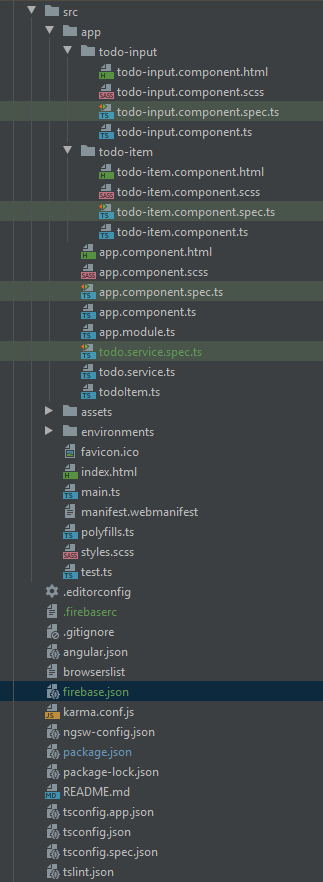
\includegraphics[scale=0.7]{img/file_tree_pwa.PNG}
	\caption{Dateistruktur des Projekts}
	\label{fig:dialog_install_pwa_desktop}
\end{figure}


\subsection{Angular}
https://www.sitepoint.com/angular-2-tutorial/
\subsection{Hinzufügen der Manifestdatei}
https://medium.com/poka-techblog/turn-your-angular-app-into-a-pwa-in-4-easy-steps-543510a9b626

\subsection{Desktop}

\begin{figure}[h]
	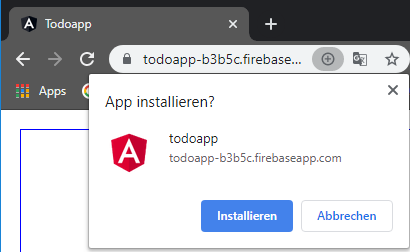
\includegraphics[scale=0.5]{img/add_to_desktop_2.PNG}
	\centering
	\caption{Browserdialog zum Installieren der PWA als Windows Desktop App}
	\label{fig:dialog_install_pwa_desktop}
\end{figure}

\begin{figure}[h]
	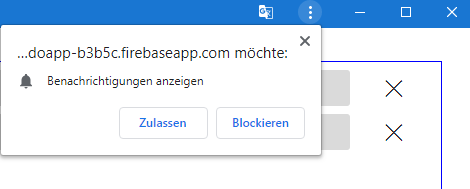
\includegraphics[scale=0.5]{img/berechtigungen_zulassen.PNG}
	\centering
	\caption{Größen}
	\label{fig:dimensions}
\end{figure}